\chapter{Upgrade of the Pixel Tracker}

The CMS detector as described in chapter \ref{chap:exp_setup} was performing during the time period 
between 2010 and 2012. It provided a center-of-mass energy up to 8 TeV and the bunch spacing was 50 ns. 
However, the LHC program was planned for at least a decade longer and the plan included several improvements.

After the shutdown for two years, from the end of 2012 until the beginning of 2015, the LHC 
center-of-mass energy was increased up to 13 TeV and will be further increased to the designed value
of 14 TeV. The next long shutdown is planned in 2018. Until that time it is planned that the peak
luminosity will reach $2 \cdot 10^{34} cm^{-2} s^{-1}$ (comparing to the $7 \cdot 10^{33} cm^{-2}s^{-1}$
reached in 2012). The total integrated luminosity which is planned to achieve prior the second long shutdown
is 200 fb$^{-1}$ \cite{CMS:2012sda}.

The plan after the second long shutdown (2018) is to increase the brightness of the bunches
in the accelerators. This is planned to be done with improving the injectors. The third long shutdown in 2022
will be used for the LHC itself improvements.

It is natural that the changes of the accelerator systems have to be reflected also in the detector construction.
If the collisions with higher energies and frequencies are provided by the accelerator machine, the detector might
be overloaded with information and some of its parts might be damaged by the higher radiation. That is why 
the CMS is also being upgraded simultaneously with the LHC.

The silicon pixel tracker (see the decription in sec. \ref{sec:tracker}) is the innermost part of the CMS 
detector mounted around the beam pipe and being the closest detector to the collision point. That means that
it receives the highest irradiation dose and operates in a very dense particle environment. After the upgrade 
in 2015 the conditions for the pixel tracker will get even more severe. That is why it has to be significantly 
upgraded to perform with the sufficient precision. 

This chapter describes the studies performed in frames of the fourth layer barrel pixel detector upgrade for the
LHC run 2015 -- 2018. It is mainly concentrated on the barrel pixel tracker, and specifically on the tests for the
planned fourth layer of the latter.

\section{Plan For the Upgrade of the Barrel Pixel Tracker}

This section will give a brief overview of the plan for the whole CMS silicon pixel upgrade in frames of so-called
Phase I upgrade. The purpose of this upgrade is to remake and update the present silicon pixel tracker to make it 
suitable for the high luminosity and energy runs which will start after the year 2016. The replacement of the silicon
pixel tracker is planned for the technical stop in 2016/2017. 

The main goal for the updated pixel detector is that it should function at higher luminosities with the same or even
better performance as the current pixel tracker on the lower luminosities \cite{CMS:2012sda}. For these needs the new read-out chips
(ROCs) have to be designed such that the data losses would be minimized. In addition, the readout system as well as all
the other detector components have to be radiation hard, as the expected doses which the detector has to meet (especially
the first layer, which is the closest to the beam pipe) are much increased.

It was also decided to increase the number of barrel layers of the pixel detector from 3 to 4 (see Fig. \ref{fig:tracker_4}).
They were designed as four concentric cylinders with the length of 548.8 mm and radii between 30 mm and 160 mm.
It would improve the track identification, which is crucial in the environment with a twice higher pile-up, expected for the 
LHC run after 2017. In addition the innermost layer of the detector is moved closer to the collision point (by 10 mm), while
the layers 2 and 3 are almost unchanged in the position. The beam pipe
will also be made smaller to allow the closer approach to the interactions.

Each layer will consist of the various number of 22 mm wide facets, each consisting of 1184 rectangular pixel modules. Each module
consists of 16 pixel chips. The total number of pixels will be increased from roughly 48 M to 79 M.

\begin{figure}[t]
 \centering
 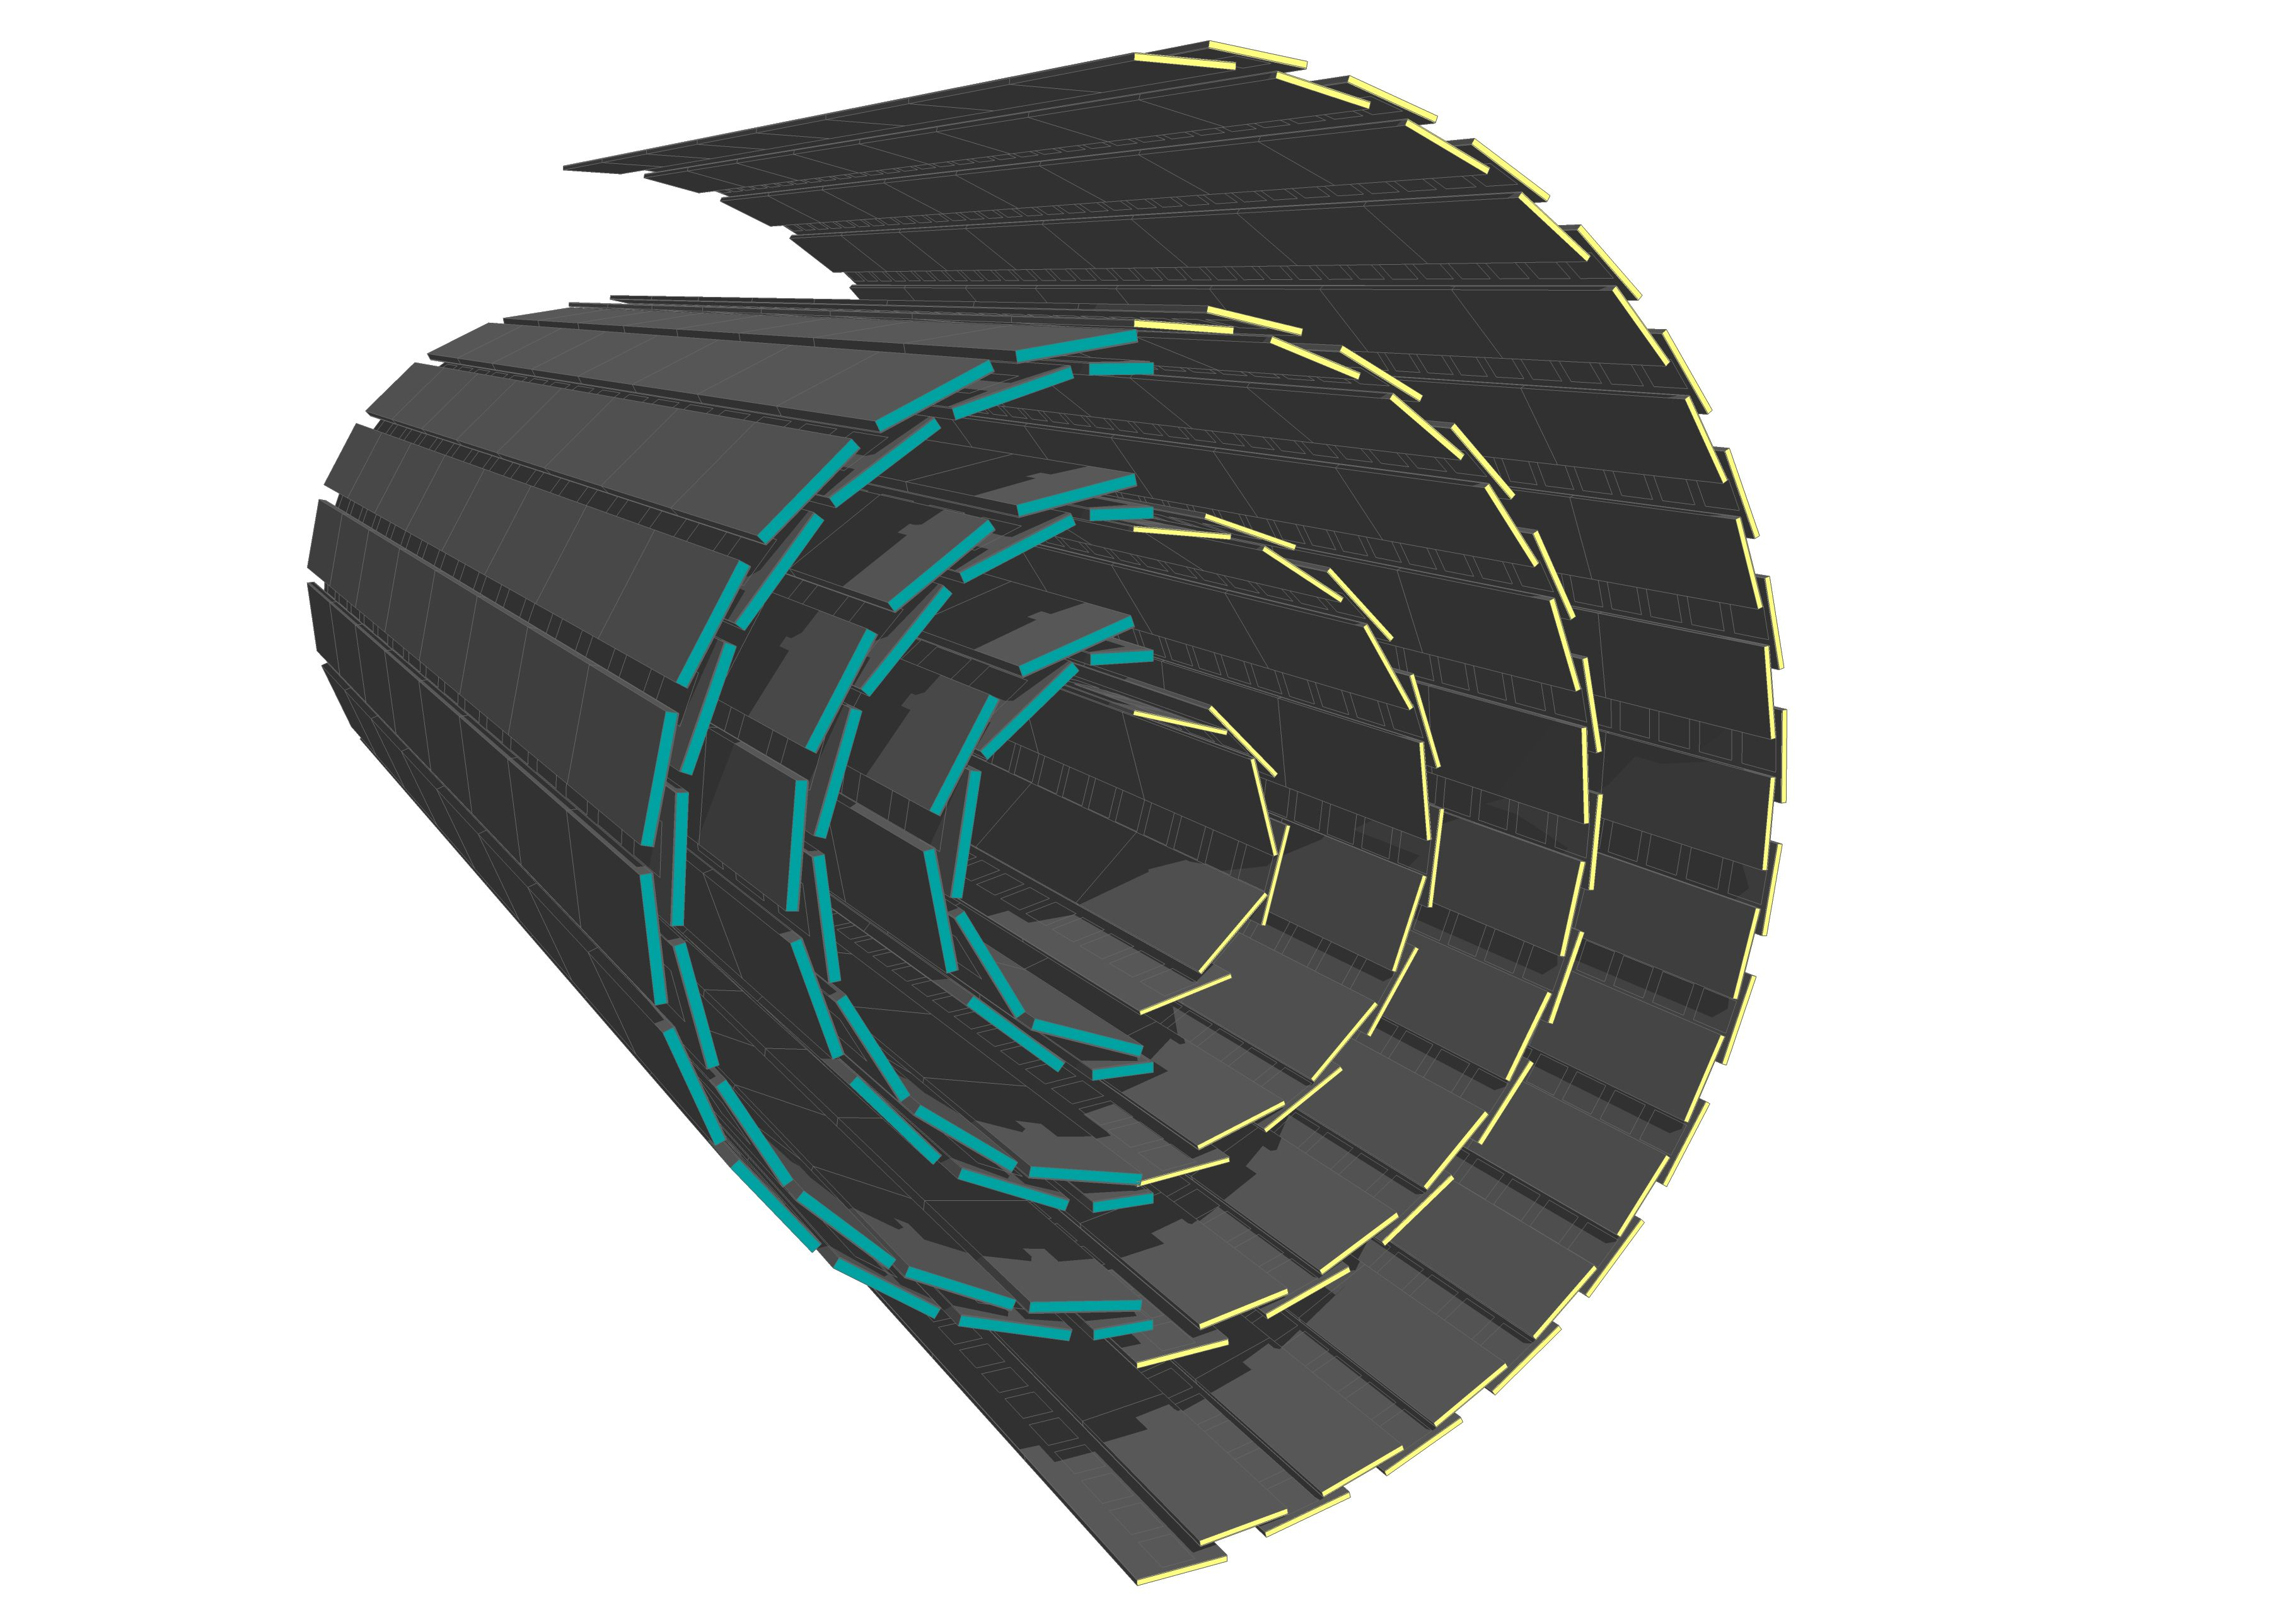
\includegraphics[width=1.0\textwidth]{021_pixel_upgrade/plots/pixel_phase1_4_layers.png}
 \caption{The model of the barrel pixel tracker before (on the left) and after the Phase 1 upgrade (on the right).}
 \label{fig:tracker_4}
\end{figure}

Addition of the fourth layer increases the amount of material which the particles have to go through. This is not
the desired feature for the innermost detectors. There are several ways planned to decrease the material amount on the 
way of the particle. So the volume of the material, which the detector is made of, has to be decreased. 
First of all, the readout system itself is planned to be thinner (it is easy to see in the Fig. \ref{fig:tracker_4},
where the new pixel barrels are thinner). And secondly, the cooling system will be changed to the $CO_{2}$ cooling \cite{CMS:2012sda} with 
light-weight mechanical support, allowing the electronic boards to be moved out of the detector volume.

The improvements planned will lead to the higher efficiencies, lower fake track rates (see sec. \ref{ssec:trkReco}), lower read-out dead time,
and extended lifetime of the detector. This results the better identification of the particles for offline analysis and HLT.

The planned upgraded detector performance was simulated. It was compared to the performance of the non-upgraded tracker. This comparison
is shown in Fig. \ref{fig:sim_perform}. These simulations were performed on the $t\bar{t}$ samples. The studies show overall higher 
efficiencies and lower fake rates for the higher pule-up scenarios.

\begin{figure}[p]
 \centering
 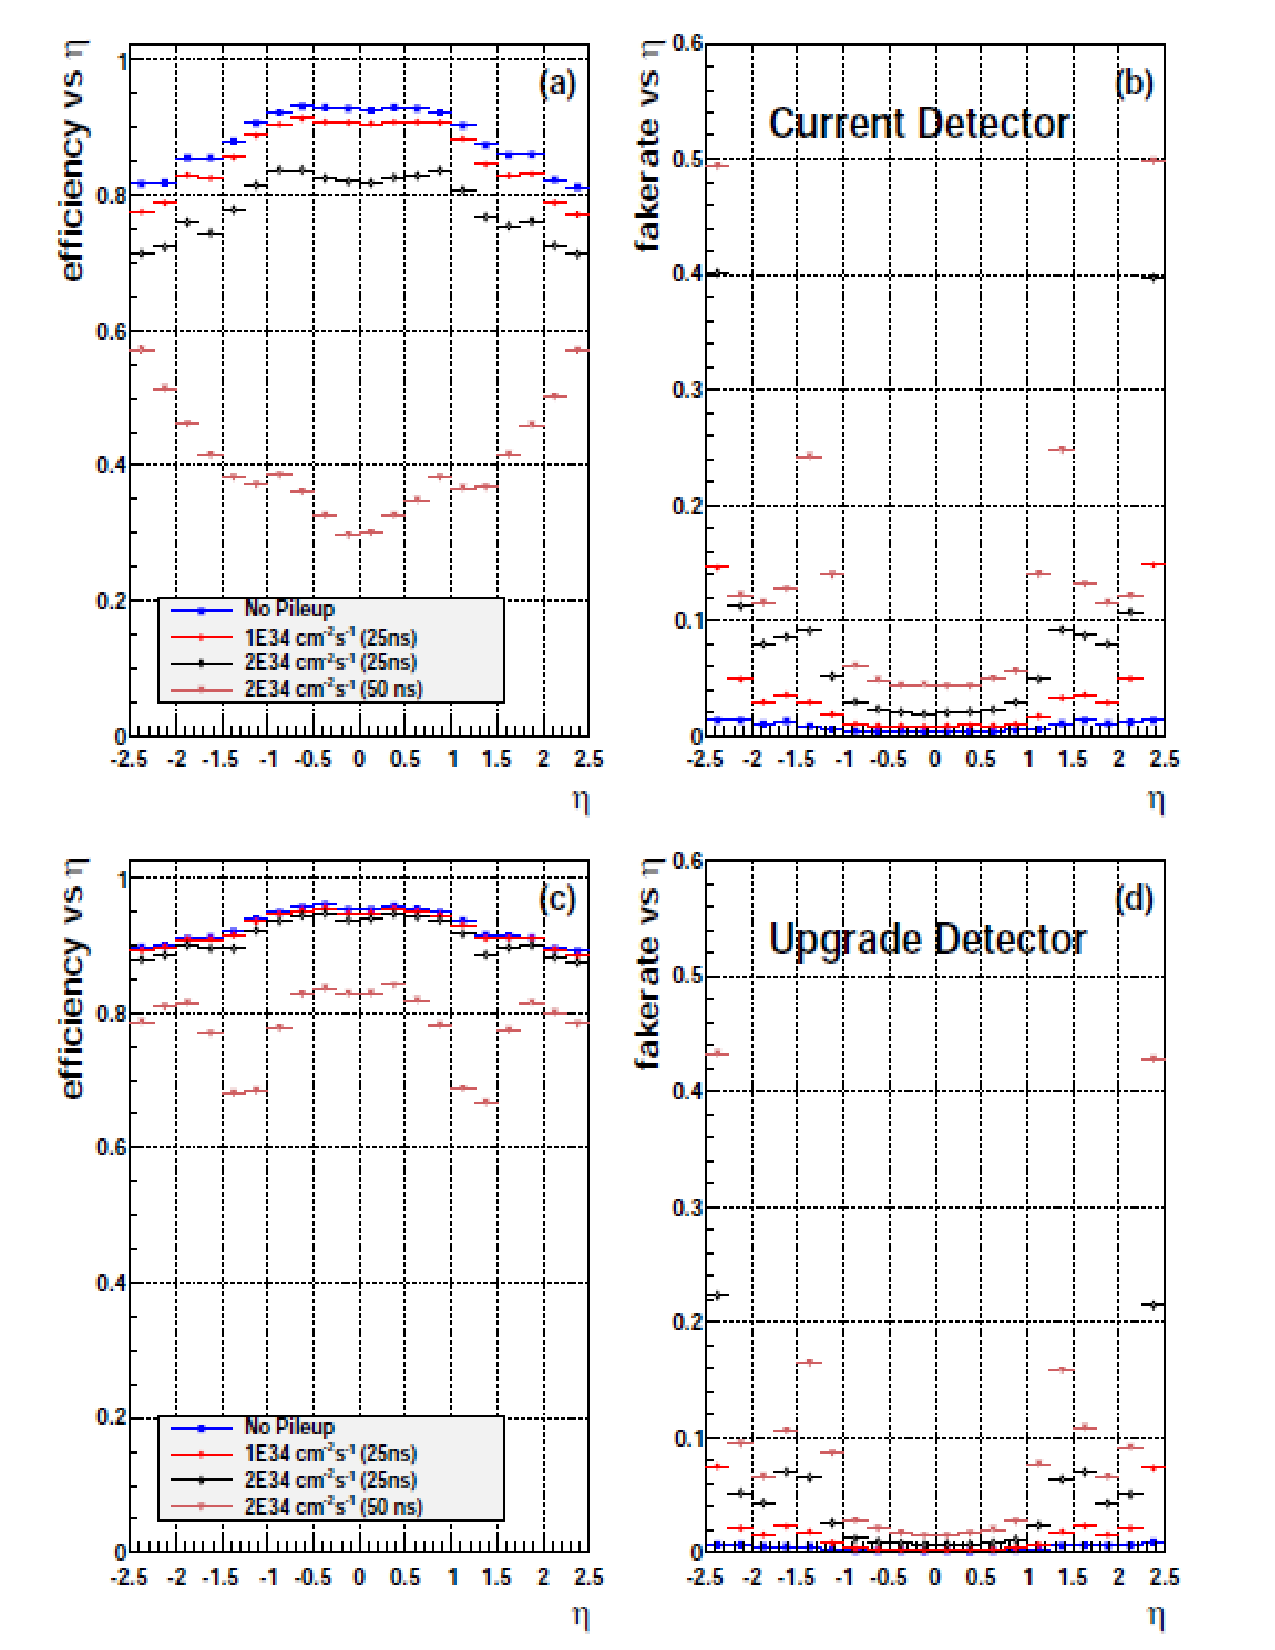
\includegraphics[width=0.8\textwidth]{021_pixel_upgrade/plots/sim_perform.pdf}
 \caption{Tracking efficiency (a,c) and fake rate (b,d) for the $t\bar{t}$ sample as a function of track
          pseudorapidity $\eta$, for the current detector (a,b) and the upgrade pixel detector (c,d). Results are shown for
          zero pileup (blue squares), an average pileup of 25 (red dots), an average pileup of 50 (black
          diamonds), and an average pileup of 100 (brown triangles) with ROC data loss simulation
          expected at the given luminosities. The plot is taken from \cite{CMS:2012sda}.}
 \label{fig:sim_perform}
\end{figure}


\section{Studies of Irradiated Prototype Modules}

The expected performance of the barrel pixel tracker was confirmed in the simulated experiments. However, it is also crucial to test 
the performance of the device under real conditions. 

The prototype single chips were produced for the needs of such tests. These are the chips of the design which was meant for the production
of the real detector facility, but supplemented with the separate readout system and board to enable an independent operation of such
a chip. 

In this work the tests of the prototype chips for the fourth layer barrel pixel (BPIX) detector. The layout of the prototype chip is shown 
in Fig. \ref{fig:prototype}. The chip is a 1/16 part of the modules from which the pixel detector will consist. 
One prototype chip contains 80 rows and 52 columns of pixels, each of the size of $100\times150$ $\mu$m$^{2}$.
These pixels collect electrons from oxygenated high-resistivity $n$-type silicon sensor of 285 $\mu$m thickness with n+ implants. 

\begin{figure}[t]
 \centering
 \begin{subfigure}
  \centering
  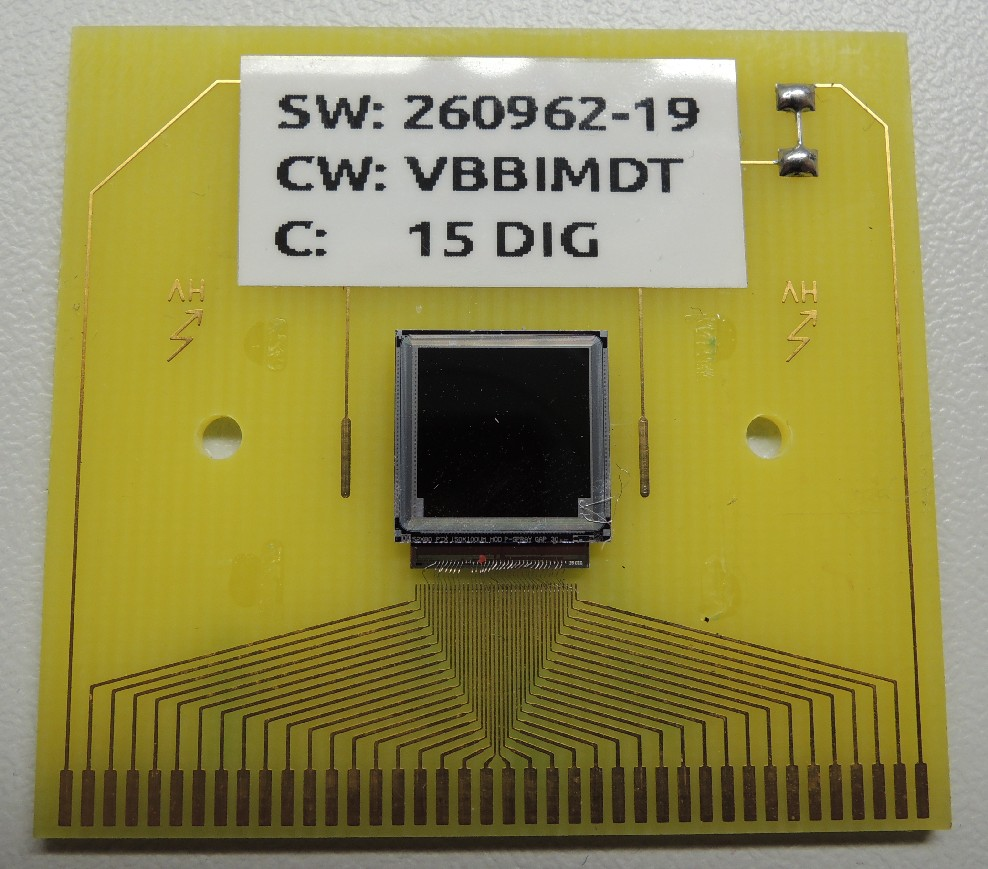
\includegraphics[width=0.4\textwidth]{021_pixel_upgrade/plots/prototype_chip_photo.png}
 \end{subfigure}
 \begin{subfigure}
  \centering
  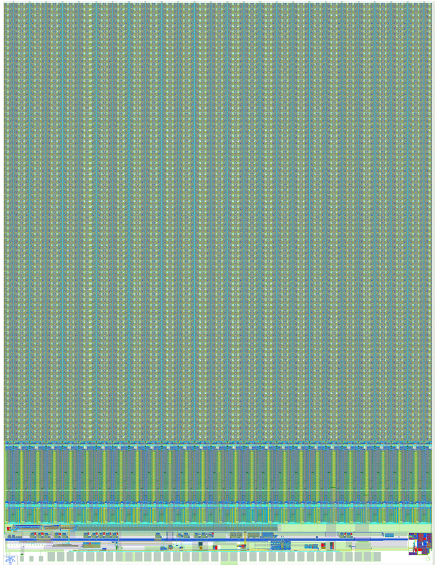
\includegraphics[width=0.4\textwidth]{021_pixel_upgrade/plots/prototype_chip.png}
 \end{subfigure}
 \caption{The photo of the prototype silicon pixel chip for the Phase I upgrade of the CMS BPIX, 4 layer, mounted to the readout panel (on the left)
 and the magnified microscope shot of the sensitive silicon pixel area (on the right).}
 \label{fig:prototype}
\end{figure}

Each pixel is bump-bonded to the ROC of the same height and width. The ROCs are fabricated in 250 nm CMOS (Complementary Metal-Oxide-Semiconductor)
employing the radiation hard design rules.
For the upgrade, the data buffer is increased to be able to work with higher occupancy connected with the higher data flow from the more frequent 
and dense LHC collisions. Furthermore the measured charges are digitalized and transmitted at 160 MHz. The effect of the internal cross talk is reduced
by design optimization and use of the 6 metal layers for the circuit, which allowed to operate at lower thresholds.

One of the important tests was to examine the chips with new design with respect to their radiation hardness. As it was discussed before, the
pixel detector will receive the maximum dose of the radiation being the closest detector part to the collision point (see Fig. \ref{fig:irrad_dose}).
It is expected that the dose absorbed by the layer 1 of BPIX during the full lifetime of the detector will be 100 MRad, or 1 MGy. Layer 2 is 
expected to absorb 40 MRad (0.4 MGy), layer 3 -- 20 MRad (0.2 MGy) and layer 4 -- 13 MRad (0.13 MGy).

\begin{figure}[t]
 \centering
 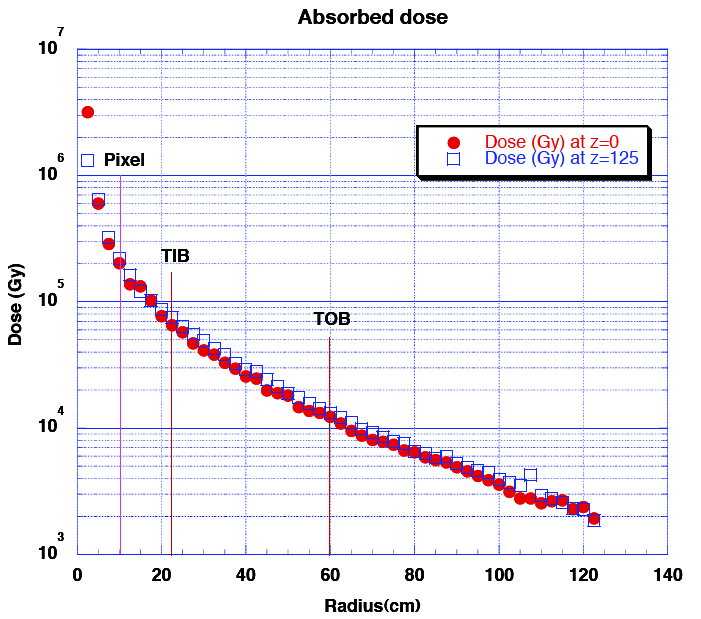
\includegraphics[width=0.8\textwidth]{021_pixel_upgrade/plots/irradiation_dose.png}
 \caption{The dose in Gy on to be received at different radial distance from the collision point for different $z$ coordinate values. The 
 average position of the pixel detector is marked with a red vertical line. The location of different parts of the silicon strip detector
 are also shown for the comparison. The dose is defined for the expected full runtime of the LHC until 2018, which corresponds to the integrated
 luminosity of 500 fb$^{-1}$.}
 \label{fig:irrad_dose}
\end{figure}

Here the studies of the properties of the irradiated prototype chips for the layer 4 of BPIX will be presented. For these needs the prototype
chips were irradiated at CERN PS [??] with the 23 GeV protons up to fluences of 3.8 $\cdot$ 10$^{14}$ $p/cm^{2}$ which corresponds to the lifetime
dose of the layer 4 of the BPIX (approximately 16 MRad). 

The prototype chips were irradiated such that the silicon sensor side was facing the beam. The readout chips on the back side received the dose
up to 130 kGy. The tests  in the laboratory at DESY \cite{DESYWeb} showed the full functionality of the irradiated ROCs.

\subsection{DESY Beam Test}

To test the functionality of the prototype silicon pixel chip, one needs to deliver some particles with relatively high energy and let
the chip register them. For these needs the so called beam tests are performed. For the studies described in this thesis, the DESY beam test
facility was exploited.

The DESY beam test facility makes use of the electron-positron synchrotron DESY II \cite{Hemmie:1982xq, DESYIIWeb}, which provides the electron
and positron beams with up to 1000 particles per cm$^{2}$ at the energies of up to 6 GeV. However, these are not the particles which are directed
to the beam test areas. The circulating DESY II beam meets the 25$\mu$m thick carbon fiber and emits bremsstrahlung. The resulting photons are afterwards 
converted to the electron-positron pairs on the converter, which is actually a metal plane. The resulting beam is passed to a dipole magnet for
separating the particles with needed momentum. Afterwards the beam is collimated and brought to the area where it can be exploited for the
experimental needs. The scheme of the facility which delivers the beam for the tests is shown in Fig. \ref{fig:desy_tb}.

\begin{figure}[t]
 \centering
 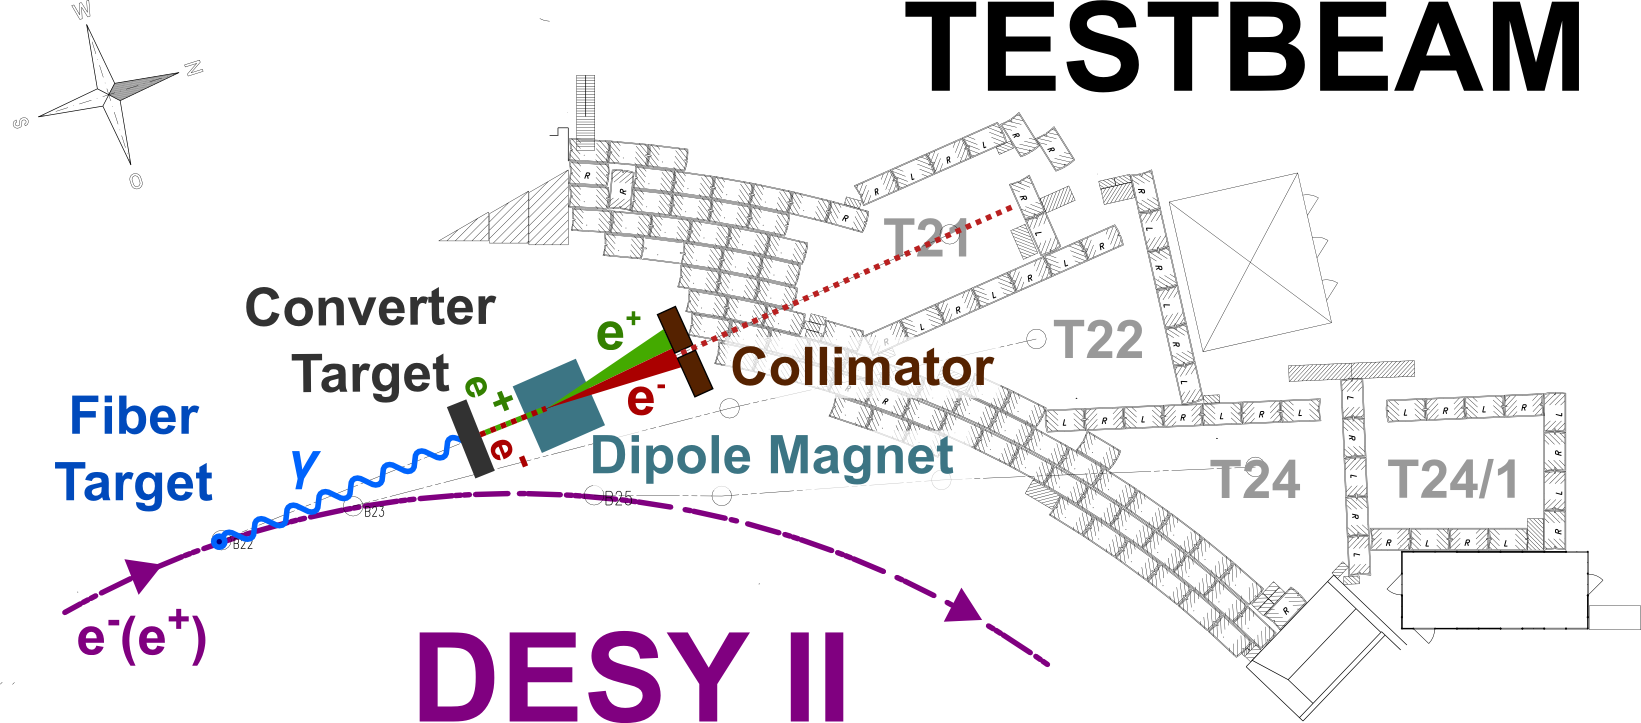
\includegraphics[width=1.0\textwidth]{021_pixel_upgrade/plots/desy_tb-sketch.png}
 \caption{Schematic layout of a test beam at DESY.}
 \label{fig:desy_tb}
\end{figure}

\subsection{EUDET Telescope and Experimental Setup} 

The beam test line where the tests described in this thesis were performed is equipped with the telescope of the EUDET/AIDA-family \cite{EUDET},
which is shown in Fig. \ref{fig:EUDET_tel}. It consists of two arms each equipped with three sensors kept at a stable temperature by a cooling
system. Each sensor plate can be moved along the beam axis to meet some particular experimental requirements.

\begin{figure}[t]
 \centering
 \includegraphics[width=1.0\textwidth]{021_pixel_upgrade/plots/Fig1.pdf}
 \caption{The photo of the EUDET telescope present at the beam test line 21 at DESY. The device under test is installed in between the two
 groups consisting of three telescope plates each. The electron/positron beam is falling perpendicularly on the EUDET telescope planes 
 from the right side of this photo.}
 \label{fig:EUDET_tel}
\end{figure}

The telescope serves as a device, which measures the particle path with a very good precision so that it is assumed to be known.
The EUDET telescope is equipped with the silicon pixels. The telescope sensors have the point precision of 2-3 $\mu$m and they
are made with a minimum of material (their thickness is only 50 $\mu$m), so that the precision doesn't drop even on the lowest 
energy border of the test beam ($\sim$ 1 GeV), when the contribution of the interaction of the particles with matter becomes 
sizable. The Mimosa (Minimum Ionazing MOS Active Pixel Sensor) sensors (of the size of $21 \times 11$ mm$^{2}$ with squared 
pixels of size of 18.4 $\mu$m) developed for the EUDET telescope made use of the MAPS (Monolitic Active Pixel Sensors) 
technology \cite{2001NIMPA.458..677T, Fischer:2002bv}.

The prototype silicon pixel chip for the BPIX upgrade was placed in between two arms of the telescope. In frames of the beam test 
campaign the device which is placed for tests (in our case it's the prototype chip) is called a device-under-test, DUT. The DUT
and it's board are placed in a special frame which allows the tilting and the turning (see Fig. \ref{fig:prototype_board}). 
This enables the studies of the detector behavior with inclined particle tracks producing multi-pixel clusters. 

\begin{figure}[t]
 \centering
 \includegraphics[width=1.0\textwidth]{021_pixel_upgrade/plots/prototype_board.png}
 \caption{The photo of DUT (prototype silicon pixel chip for the BPIX 4$^{th}$ layer upgrade) and it's board in the metal frame
 mounted between two arms of the EUDET telescope at the DESY beam test area.}
 \label{fig:prototype_board}
\end{figure}

There is a second CMS prototype chip placed downstream at the end of the beam telescope. It had to serve as a reference for the
measurement of the DUT efficiency.

On the front before and in the end right after the telescope plains two crossed scintillators are located. They serve as a trigger. 
If their signals coincide, the particle has passed all the way through the telescope.
The typical duration of one run when the telescope, DUT and reference chip were registering the test beam particles, was from 10
to 30 minutes having several hundred thousand trigger signals.

\subsection{Data Taking}

The data from the telescope was passed to the computer through the network cables (see Fig. \ref{fig:EUDET_tel}) and from
the CMS prototype chips -- through the USB cables (see Fig. \ref{fig:prototype_board}). These are the signals, which inform
about the particles hit the detector plane.  Afterwards the received data had to be preanalysed. 

To gain the better knowledge of the geometry of the setup, the alignment procedure is done. The alignment was done with the
Millipede algorithm \cite{1748-0221-3-09-P09002}.

The neighboring fired pixels on the pixel detector are grouped into clusters.

The tracks were reconstructed using the general broken lines algorithm \cite{Blobel:2006yi}. It takes the multiple scattering
in the detector planes into account. The particle track is reconstructed using the hits in the first and third telescope planes.
The second plane is used for the telescope hit resolution determination from the difference between the reconstructed particle
track position and the actual hit in the second telescope plane. This resolution is stable from run to run and results about
3.5 $\mu$m.

This basic information from the telescope and from the prototype chips is used for the further analysis.

\subsection{Analyzing the Prototype Chip Properties}

Several crucial properties which are important for the future BPIX detector operation were measured using the data taken from the 
tests on the DESY beam test.

\subsubsection{Charge Collection}

The external bias voltage is needed to collect all the charge which was released due to the particle crossing the sensitive silicon
pixel of the detector. If the bias voltage is not high enough, not all the charge is collected and the particle energy may be defined
incorrectly. The voltage at which the full charge starts to be collected is called \textit{depletion voltage}. The bias voltage is
applied on the $p$-implant side. The schematic path of the ionizing particle through the silicon sensor is displayed at the following sketch:

\begin{figure}[h]
 \centering
 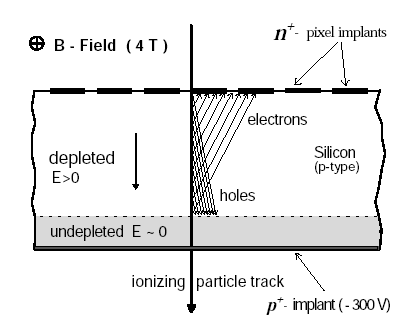
\includegraphics[width=0.6\textwidth]{021_pixel_upgrade/plots/depletion_voltage.png}
 \caption{The sketch of the charge collection from the ionizing particle crossing the silicon sensor.}
 \label{fig:depl_volt}
\end{figure}

After the irradiation the damages in the silicon material are introduced. These damages may trap the ionized charge  which is traveling 
through the silicon to the place where it is read off. That is why a higher voltage is needed so that the particles overcome the traps.
However, there is a practical power dissipation related with the ohmic heating and on the bias voltage supply. If the depletion voltage
is higher than these limitations, the full depletion conditions for the sensors can never be reached. That is why it is necessary to test
if the full depletion region can be reached and if so, then at which bias voltage.

To study this problem, the external bias voltage was varied from the very low values up to few hundred volts. The collected charge was
measured for each value of supplied bias voltage.

Fig. \ref{fig:depletion_voltage} shows the collected pixel cluster charge normalized to the maximum charge collected and tracking efficiency
of two prototype chip. These chips were irradiated to the doses of $0.9 \cdot 10^{14}$ p/cm$^2$ and $3.8 \cdot 10^{14}$ p/cm$^2$. 
The tracking efficiency was defined as the number of tracks which were registered in telescope, reference and DUT chips over the number
of tracks registered in telescope and reference chip.

\begin{figure}[t]
\centering
\begin{subfigure}
  \centering
  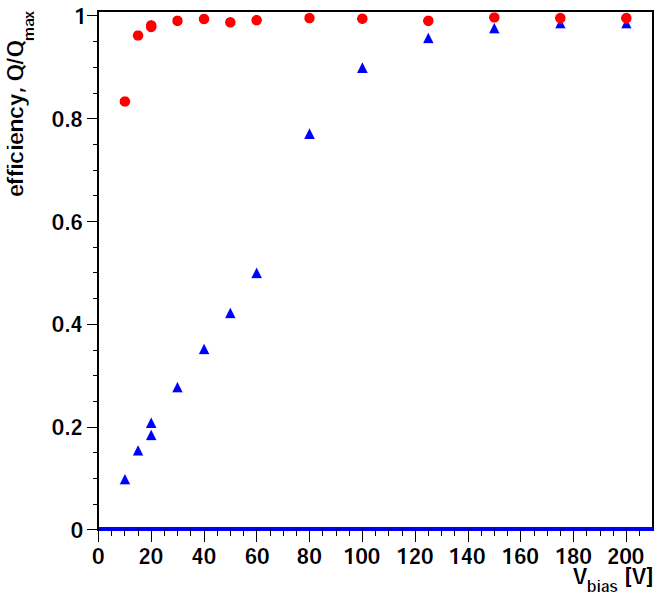
\includegraphics[width=0.42\textwidth]{021_pixel_upgrade/plots/voltage_scan_low_irrad.png}
\end{subfigure}
\begin{subfigure}
  \centering
  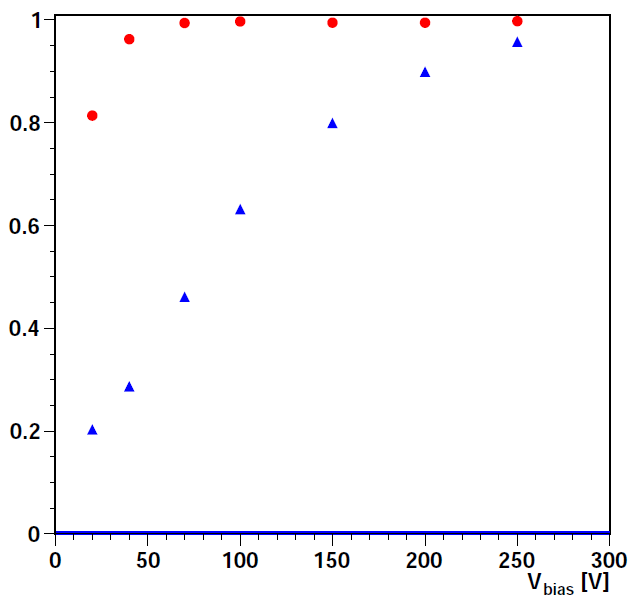
\includegraphics[width=0.4\textwidth]{021_pixel_upgrade/plots/voltage_scan_high_irrad.png}
\end{subfigure}
\caption{Charge collection efficiency, normalized to the maximum cluster charge (triangles) and tracking efficiency (circles) of the prototype silicon sensor
         for the CMS pixel tracker irradiated to $0.9 \cdot 10^{14}$ p/cm$^2$ (left) and $3.8 \cdot 10^{14}$ p/cm$^2$ (right) as function of applied bias voltage.}
\label{fig:depletion_voltage}
\end{figure}

For the prototype chip, which was irradiated to$0.9 \cdot 10^{14}$ p/cm$^2$, the collected charge drops quickly for bias voltages below -110 V. 
Only about one third of the charge is collected with the bias voltage lower than -30 V. However the tracking efficiency still remains higher
than 90\%. This means, that the detector is fully efficient in terms of tracking with only one third of the charge collected.

The chip with higher dose of $3.8 \cdot 10^{14}$ p/cm$^2$. There the full depletion is reached only with -250 V. The full tracking efficiency
is reached at -70 V, where around half of the charge was collected.

Additionally, the absolute pixel cluster charge distribution for the chip irradiated with the dose of $3.8 \cdot 10^{14}$ p/cm$^2$ was measured
with the -250 V bias voltage supplied (see Fig. \ref{fig:Landau}). It has an expected Landau shape, peaking at 18 ke. Before the irradiation a 
similar test was performed for this chip. The Landau peak was at 22 ke then. It means that there is a charge loss due to trapping in the silicon
bulk after the irradiation.

\begin{figure}[t]
 \centering
 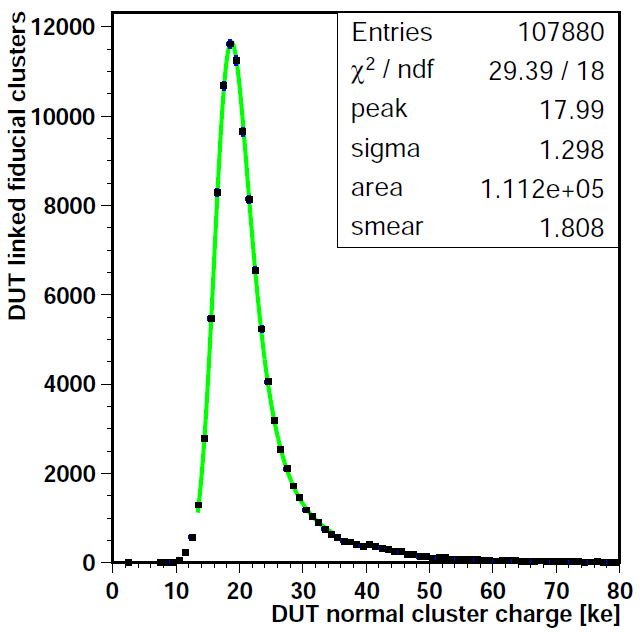
\includegraphics[width=0.6\textwidth]{021_pixel_upgrade/plots/Landau.png}
 \caption{Cluster charge distribution measured in the electron beam for a 285$\mu$m thick pixel sensor irradiated to $3.8 \cdot 10^{14}$ p/cm$^2$ 
 at a bias voltage of -250 V (plateau region).}
 \label{fig:Landau}
\end{figure}

\subsubsection{Position Resolution}

The accuracy of the measurement of the position where the particle hit the silicon detector is primarily limited by the size of the silicon pixels.
However there are ways to improve the resolution. 